%@ chapter=2
%@ exercise=8
%@ author=Fabian

The axiom of choice states that every epimorphism splits.

Given objects $P, X, E$, an arrow $f : P → X$ and an epimorphism $e : E → X$ in $\cat{Set}$, the axiom of choice gives us $e^{-1}$ in the following diagram such that $e ∘ e^{-1} = id_X$.

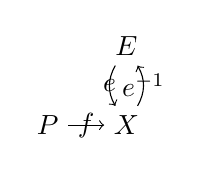
\begin{tikzpicture}
  \node (P) {$P$};
  \node (X) [right of=P] {$X$};
  \node (E) [above of=X] {$E$};
  \draw[->] (P) to node {$f$} (X);
  \draw[->, bend right] (E) to node {$e$} (X);
  \draw[->, bend right] (X) to node {$e^{-1}$} (E);
\end{tikzpicture}

We construct $\overline{f} : P → E$ so that the following diagram commutes.

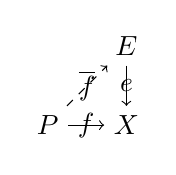
\begin{tikzpicture}
  \node (P) {$P$};
  \node (X) [right of=P] {$X$};
  \node (E) [above of=X] {$E$};
  \draw[->] (P) to node {$f$} (X);
  \draw[->] (E) to node {$e$} (X);
  \draw[->, dashed] (P) to node {$\overline{f}$} (E);
\end{tikzpicture}

$\overline{f} := e^{-1} ∘ f$ obviously does the job and $P$ is projective. Since $P$ was chosen arbitrarily every set is projective.
